\section{Usability Report}
\subsection{Process}
In order to conduct the usability study, our team used the human computer interaction experts at the University of Wisconsin-Madison HCI Lab. Our client contacted 5 experts and they reviewed our prototype system. Before the experts could review our system, they had to agree to an Informed Consent Form that is included below. A list of tasks was then provided to the experts with instructions to fill out a questionnaire on Google Documents. The questionnaire included the Informed Consent Form at the top of the form and by submitting the questionnaire the experts were agreeing to the terms of the Informed Consent Form. The specific instructions given to the experts are included below as well. Once the experts had completed the tasks, they filled out the questionnaire here \url{https://docs.google.com/spreadsheet/viewform?formkey=dExyUjl2cGJiMUlfb0dfMkFNT1k1UEE6MQ} and the questions have been copied below. This process proved to be useful since we did not have to find a common meeting time for everyone and the experts could complete the tasks on his or her own time.

\subsubsection{Informed Consent Form}
Please read this informed consent document carefully before you decide to participate in this study.

The purpose of this study is to analyze and test the design of the proposed Participant Scheduling System for use at the Human-Computer Interaction Lab at the University of Wisconsin in Madison (henceforth HCI lab).

This study is being conducted by Trey Cahill, Chris Gropp, Samad Jawaid, and Kevin Risden, with additional support from Sriram Mohan, Jimmy Theis, and Allie Terrell (henceforth the study organizers). No other persons or agencies will assist in this study or be allowed access to any identifying information.

This study is confidential; your name and specific responses will not be available to anyone outside of the study organizers. Only aggregate information will be available to the general public, and your name will not be released in any capacity (as part of a list or otherwise) to anyone outside of the study organizers.

Your specific responses and any identifying information will be destroyed no later than June 2012, even amongst the records of the study organizers.

Your participation in this study is entirely voluntary. You may refuse to answer any questions posed, and may choose to stop participating at any time.

If you have questions about the study, please contact Kevin Risden by email at risdenkj@rose-hulman.edu

Your completion and submission of the questionnaire indicates your consent to participate in this study under the terms stated above.

\subsubsection{Expert Instructions}
Thanks so much for agreeing to help out with this usability study. As you saw in my previous email, this is for the participant scheduling system for the lab and is being completed as part of a class project by a team of students from my undergraduate school. Kevin Risden (who is heading the team working on this) is CCed on this email - please feel free to email him with any questions (CC me), or if you have further comments after completing the study.

The study should take about 30 minutes to complete - instructions are below this message. Note that there is a feedback form as well via Google Docs. Since this is part of a class, the team needs your responses by Thursday morning so they can complete their milestone. Additionally, I will be out of town all day Thursday. I've asked Kevin to send out a reminder email if he doesn't have all of the responses by then.

Keep in mind that this is a prototype - their winter quarter will be spent developing the working system. So, provide constructive feedback for the team, particularly regarding the design and functionality.

Prototype: http://pss.csse.rose-hulman.edu/

Below is a provided username and password to use to login to the system.\\
Username: aterrell\\
Password: temp123

Before attempting to complete the tasks below, spend a few minutes exploring the system to gain an understanding of it.

As a HCI Lab Researcher, here is the list of tasks to complete:
\begin{itemize}
\item Login
\item Add Experiment
\item Modify Experiment
\item Experiment Time and Date Range
\item Delete Experiment
\end{itemize}

Please complete a feedback form at https://docs.google.com/spreadsheet/viewform?formkey=dExyUjl2cGJiMUlfb0dfMkFNT1k1UEE6MQ as you proceed through the tasks.

Limitations:\\
Signup will not work due to verification emails not being allowed outside the Rose-Hulman Institute of Technology firewall.

\subsubsection{Questionnaire}
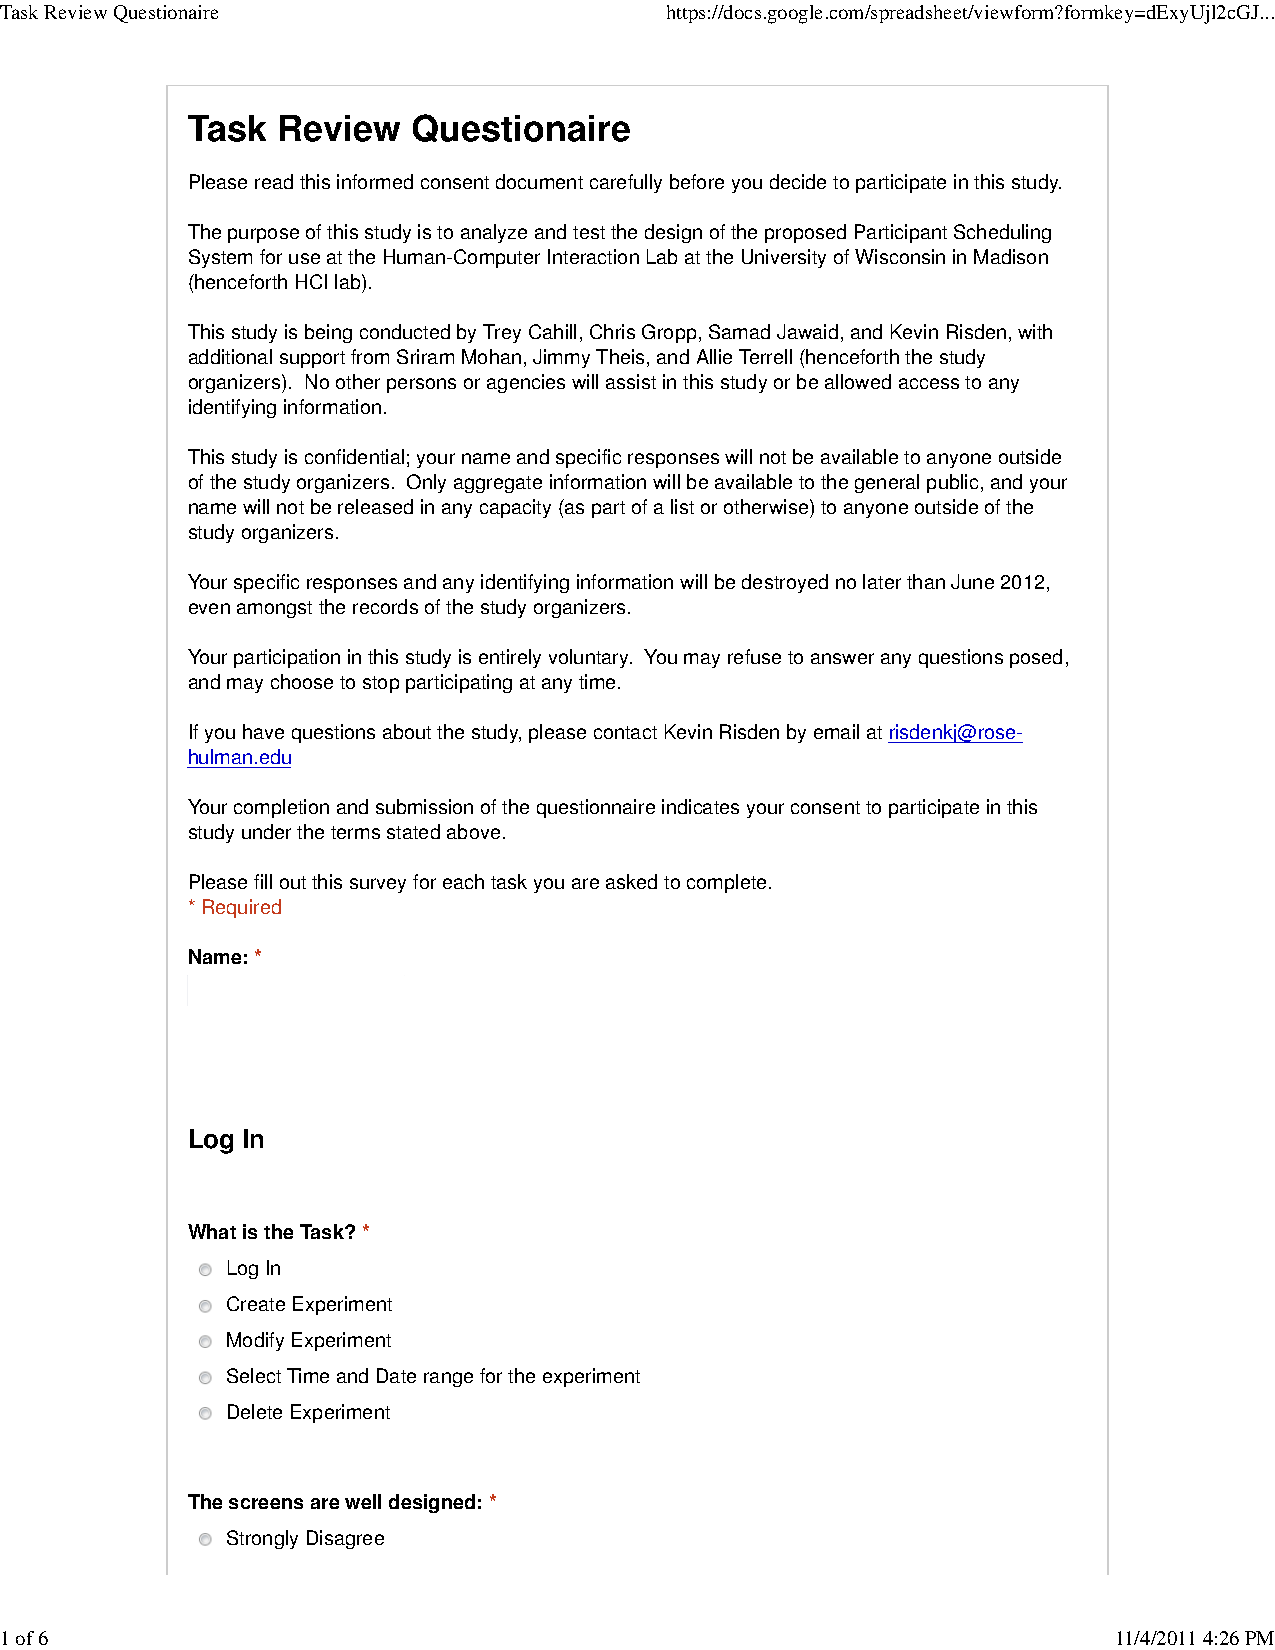
\includepdf[pages=1-,pagecommand={}]{../other/google_docs_questionnaire}

\subsection{Analysis}
Using the Google Documents form and corresponding spreadsheet provided a convenient way to aggregate the data and analyse it. The raw data was downloaded from Google Docs in Excel format and then the analysis of each task was done following the general structure outlined here:
\begin{itemize}
\item A bar chart showing the number of each type of response for how well the screen was designed.
\item The answers for the how well screen(s) were designed question were given a numerical value. Strongly disagree was given a 1, disagree a 2, neutral a 3, agree a 4, and strongly agree a 5. These scores were averaged to give an overall score for how well each task was designed in terms of the screens.
\item Common themes for the two open ended questions were identified.
\end{itemize}
The three open ended questions at the end of the questionnaire relating to the overall feel of the system were each analysed for common themes. Based on the feedback from each participant, follow-up questions were generated in order to gain more specific information.

\subsubsection{Login}
\textbf{The screen was well designed}\\
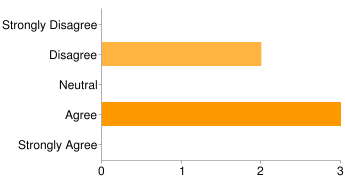
\includegraphics[page=1,scale=0.65]{../other/usability-report-charts/login_bar_chart}\\
\textbf{Average Score:} 3.2\\
\textbf{Common Themes:}
\begin{itemize}
\item Positive
\begin{itemize}
\item Simple
\item Clean
\item Straightforward
\end{itemize}
\item Negative
\begin{itemize}
\item Main page needs more content
\end{itemize}
\end{itemize}

\subsubsection{Add Experiment}
\textbf{The screen was well designed}\\
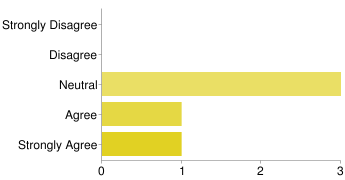
\includegraphics[page=1,scale=0.65]{../other/usability-report-charts/create_experiment_bar_chart}\\
\textbf{Average Score:} 3.6\\
\textbf{Common Themes:}
\begin{itemize}
\item Positive
\begin{itemize}
\item Intuitive
\item Style of page/buttons
\end{itemize}
\item Negative
\begin{itemize}
\item Combine Add Experiment with Date/Time Range selection
\item Add Save button to top of page
\end{itemize}
\end{itemize}

\subsubsection{Modify Experiment}
\textbf{The screen was well designed}\\
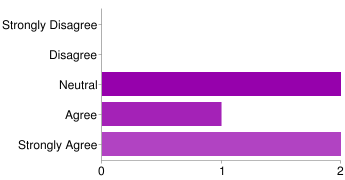
\includegraphics[page=1,scale=0.65]{../other/usability-report-charts/modify_experiment_bar_chart}\\
\textbf{Average Score:} 4\\
\textbf{Common Themes:}
\begin{itemize}
\item Positive
\begin{itemize}
\item Easy to use
\item Straightforward
\end{itemize}
\item Negative
\begin{itemize}
\item Combine Add Experiment with Date/Time Range selection
\item Modify button on list experiments page
\end{itemize}
\end{itemize}

\subsubsection{Experiment Time and Date Range}
\textbf{The screen was well designed}\\
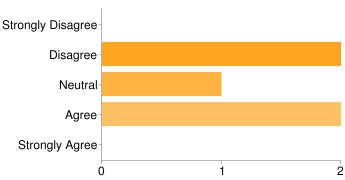
\includegraphics[page=1,scale=0.65]{../other/usability-report-charts/select_experiment_date_time_bar_chart}\\
\textbf{Average Score: 3}\\
\textbf{Common Themes:}
\begin{itemize}
\item Positive
\begin{itemize}
\item Entering time is clear and simple
\end{itemize}
\item Negative
\begin{itemize}
\item Combine Add Experiment with Date/Time Range selection
\item Use Google Calendar type interface
\item Cannot range over multiple days at once
\item Forced to use widget to enter time
\end{itemize}
\end{itemize}

\subsubsection{Delete Experiment}
\textbf{The screen was well designed}\\
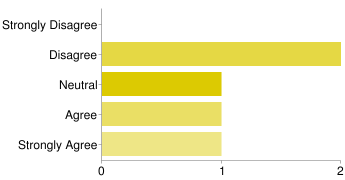
\includegraphics[page=1,scale=0.65]{../other/usability-report-charts/delete_experiment_bar_chart}\\
\textbf{Average Score:} 3.2\\
\textbf{Common Themes:}
\begin{itemize}
\item Positive
\begin{itemize}
\item Confirmation before actually deleting
\end{itemize}
\item Negative
\begin{itemize}
\item Add delete ability to list all experiments page
\item Delete button hidden
\end{itemize}
\end{itemize}

\subsection{Findings}
The analysis of the usability study provided some results that were expected due to the level of the prototype, but also some results that were unexpected. Overall findings are listed first followed by the findings broken out into the tasks the experts completed.

\subsubsection{Overall}
The experts' opinions in general showed that the prototype showed promise and the parts that were completed had only some minor issues. For each task, the average score was at or above 3 meaning that the experts either were neutral or agreed with our design. The biggest issue was the separation of experiment length and date from the experiment time slot creation. Aside from that, the minor issues included not having a meaningful home page, changing the colours of the delete experiment button, and providing indication in the top navigation bar as to what page you are on. Many of the changes suggested were already on the roadmap to be completed in the next revision. This shows that our product is on the right track and that we have done a good job relating to usability this far.

\subsubsection{Login}
The overall sentiment showed that the experts liked the simplicity of the home page and login page. The other suggestion was that the home page should provide information about the lab, which is planned for a later version when the experiments are displayed on the home page for participants to choose from. With the overall average rating being a 3.2, the experts were close to neutral due to the lack of content on the home page, but this was planned to be changed when more of the system is implemented.

\subsubsection{Add Experiment}
The comments for the Add Experiment question suggested that the division of creating an experiment and the time slots separately was a bad design. This should be integrated into one screen since the two activities are related. The ability to add rooms, qualifications, and researchers while creating an experiment is a feature that was missing from the initial prototype but is on the radar to be completed in the next revision. This hurt the usability since the experts could not create a new room or add a qualification. One comment related to not knowing what a qualification was and we attribute this to not using the same terminology when they create an experiment. If this is a common theme with later studies, we may look into changing the wording. The positive attributes of the Add Experiment task was that it was straightforward and that the interface had a nice pleasing layout to the eye.

\subsubsection{Modify Experiment}
Much of the feedback for Modify Experiment mirrored the Add Experiment feedback since they were similar in the page design. Since the two designs are similar the fixes for Add Experiment will also apply to the Modify Experiment task. There was some more positive feedback for the Modify Experiment page such as providing a green line when modifying the experiment was a good indicator. Another good design feedback was that the experts liked the modify button the side of the experiment list. On the downside, the delete button was too hidden and hard to find when needed. The next revision plans to fix the delete button issue and is addressed more in the Delete Experiment task.

\subsubsection{Experiment Time and Date Range}
The Experiment Time and Date Range had varied feedback since some users liked the use of military time for entering the time but others wanted a Google Calendar type approach to entering the time. In addition to this, some of the experts wanted the ability to type in a date and time instead of being forced to use the calendar and time widgets. The important critical feedback we received was that the experts did not like having the Experiment Time and Date Range task separate from the Create/Modify Experiment task. They felt that this is the same task and should be handled on one screen instead of two separate screens. This feedback means that we need to redesign how the time and date ranges are chosen for our next releases of the prototype.

\subsubsection{Delete Experiment}
The major issue pointed out during the Delete Experiment task was that the delete button was hard to impossible to find. It did not match the look and feel of the other buttons on the site and this made it a difficult button to find. The experts felt that button should be more subtle than the save button but still fit the look and feel of the other buttons. Another suggestion was to include a way to delete experiments from the experiment list instead of having to open an experiment first. The positive feedback was that deleting an experiment was straightforward once the delete button was found. The next revision was planned to redesign the way the delete button worked so now we know how the delete button should be redesigned based on the expert feedback.